\section{Discussion}
\label{sec:discussion}
    
    
    % \begin{figure}
    %     \centering
    %     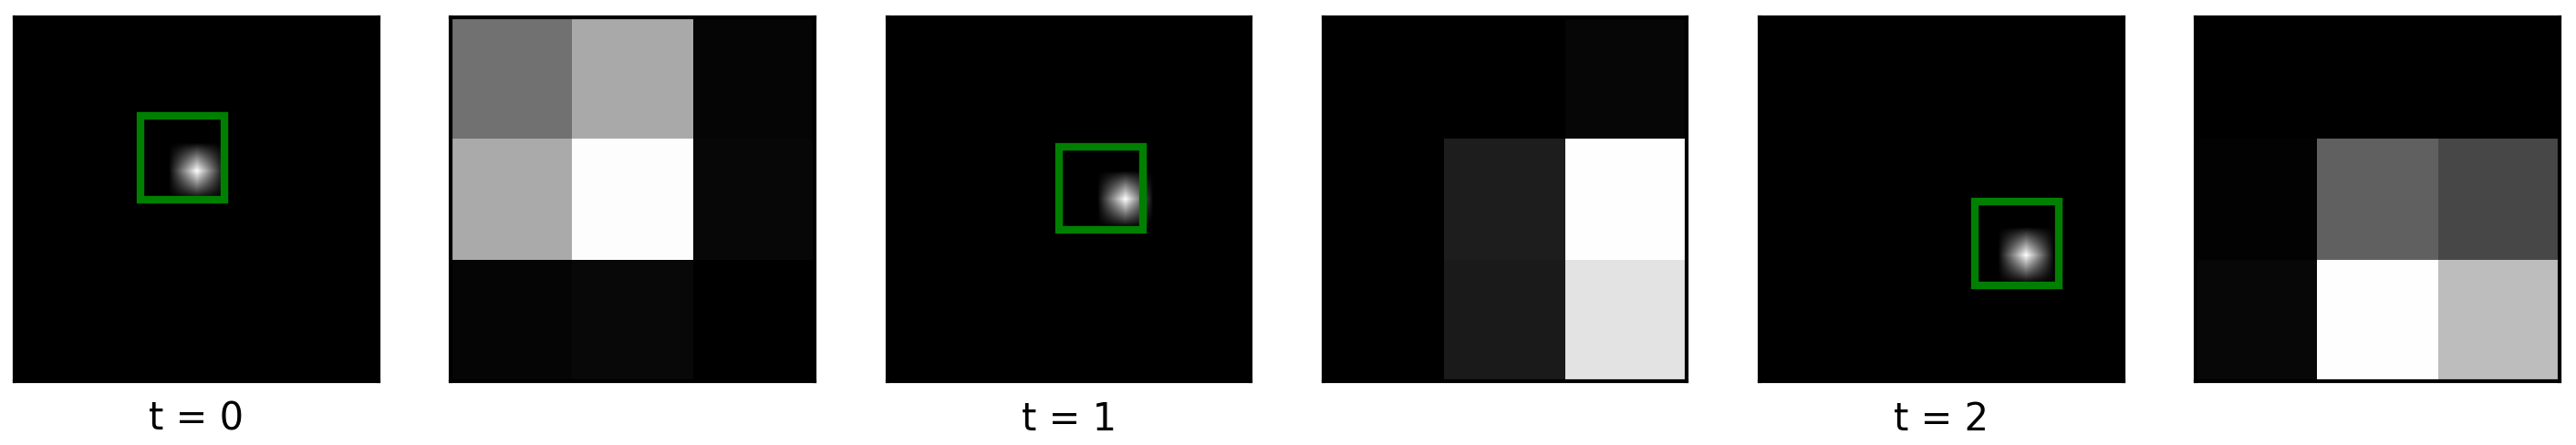
\includegraphics[width=\textwidth]{att_loss_expr}
    %     \caption{Setup for tracking a single white dot on a black background. This simple setup allows to evaluate influence of different loss components on learning.}
    %     \label{fig:att_min_setup}
    % \end{figure}
    
      \begin{figure}
      \centering
      \begin{subfigure}[b]{\textwidth}
        \centering
        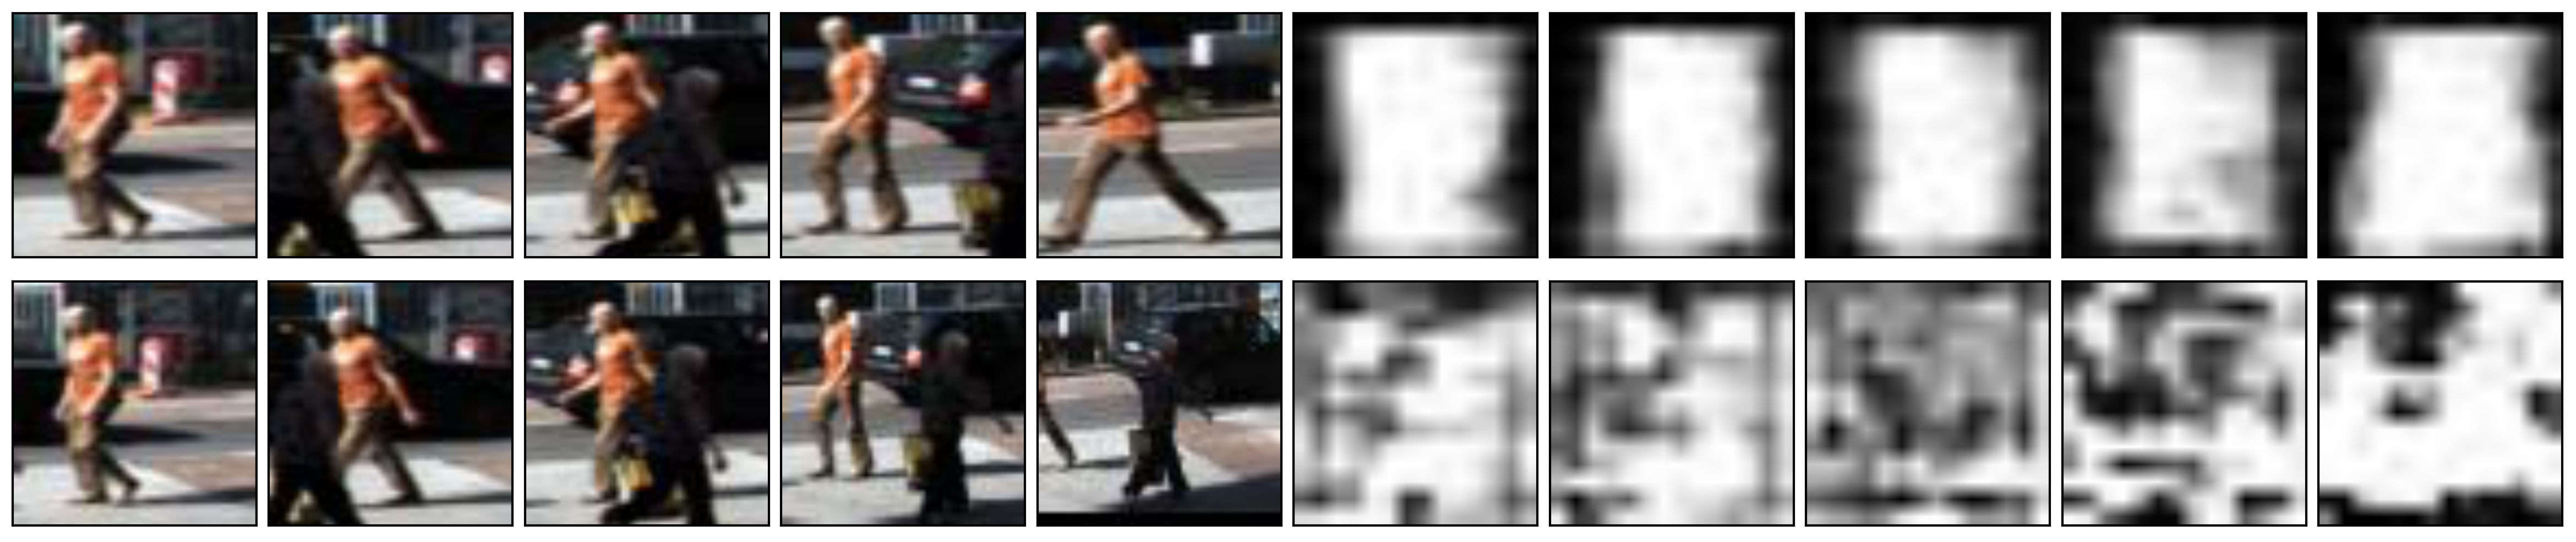
\includegraphics[width=\textwidth]{HART/soft_id_swap}
        \subcaption{The model with appearance attention loss (top) learns to focus on the tracked object, which prevents an ID swap when a pedestrian is occluded by another one (bottom).}
        \label{fig:soft_id_swap}
      \end{subfigure}
      
      \begin{subfigure}[b]{\textwidth}
        \centering
        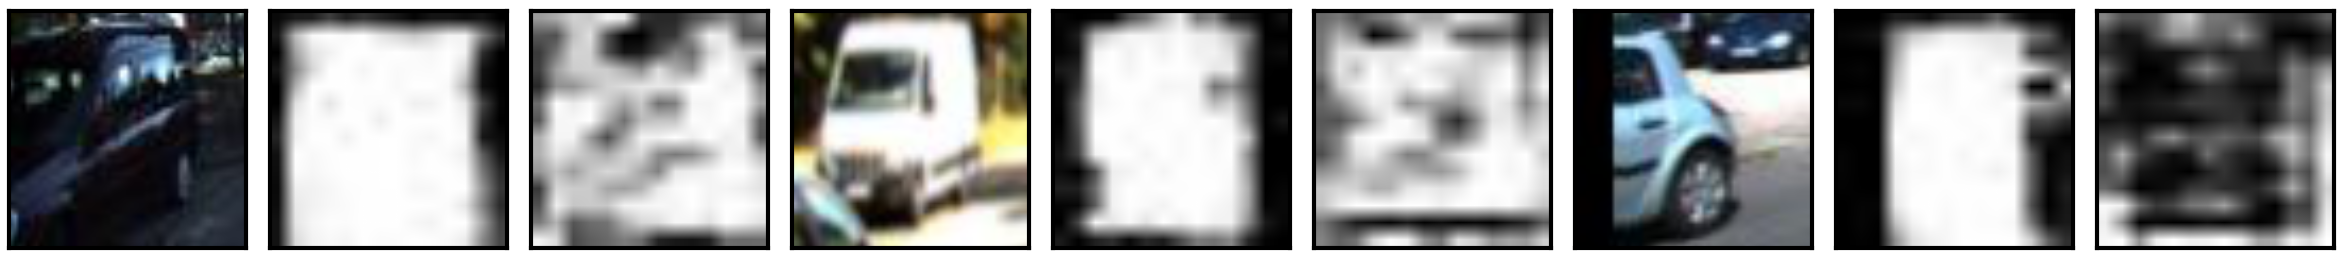
\includegraphics[width=\textwidth]{HART/soft_att}
        \subcaption{Three examples of glimpses and locations maps for a model with and without appearance loss (left to right). Attention loss forces the appearance attention to pick out only the tracked object, thereby suppressing distractors.}
        \label{fig:soft_att_examples}
      \end{subfigure}
      
      \caption{Glimpses and corresponding location maps for models trained with and without appearance loss. The appearance loss encourages the model to learn foreground/background segmentation of the input glimpse.}
      \label{fig:soft_att}
    \end{figure}
    
  
    The experiments in the previous section show that it is possible to track real-world objects with a recurrent attentive tracker. While similar to the tracker by \citet{Kahou2015ratm}, our approach uses additional building blocks, specifically: 
%    \begin{enumerate*}[label=(\roman*)]
	\begin{inparaenum}[(i)]
        \item bounding-box regression loss,
        \item loss on spatial attention,
        \item appearance attention with an additional loss term, and
        \item combines all of these in a unified approach.
%    \end{enumerate*}
	\end{inparaenum}
    We now discuss properties of these modules.
    \begin{description}[leftmargin=\parindent]
        \item[Spatial Attention Loss prevents Vanishing Gradients]        
        Our early experiments suggest that using only the tracking loss causes an instance of the vanishing gradient problem. Early in training, the system is not able to estimate object's motion correctly, leading to cases where the extracted glimpse does not contain the tracked object or contains only a part thereof. In such cases, the supervisory signal is only weakly correlated with the model's input, which prevents learning. Even when the object is contained within the glimpse, the gradient path from the loss function is rather long, since any teaching signal has to pass to the previous timestep through the feature extractor stage. Penalising attention parameters directly seems to solve this issue.
        
        \item[Is Appearance Attention Loss Necessary?]
        Given enough data and sufficiently high model capacity, appearance attention should be able to filter out irrelevant input features before updating the working memory. In general, however, this behaviour can be achieved faster if the model is constrained to do so by using an appropriate loss. \Cref{fig:soft_att} shows examples of glimpses and corresponding location maps for a model with and without loss on the appearance attention. In \cref{fig:soft_id_swap} the model with loss on appearance attention is able to track a pedestrian even after it was occluded by another human. \Cref{fig:soft_att_examples} shows that, when not penalised, location map might not be very object-specific and can miss the object entirely (right-most figure). By using the appearance attention loss, we not only improve results but also make the model more interpretable.
    
        \item[Spatial Attention Bias is Always Positive]
        To condition the system on the object's appearance and make it independent of the starting location, we translate the initial bounding box to attention parameters, to which we add a learnable bias, and create the hidden state of LSTM from corresponding visual features. In our experiments, this bias always converged to positive values favouring attention glimpse slightly larger than the object bounding box. It suggests that, while discarding irrelevant features is desirable for object tracking, the system as a whole learns to trade off attention responsibility between the spatial and appearance based attention modules.
        
        
    \end{description}